\documentclass[crop,tikz]{standalone}

\usepackage{pgfplots}
\tikzset{>=latex}
\usetikzlibrary{calc}

\colorlet{green}{black!40!green}

\begin{document}
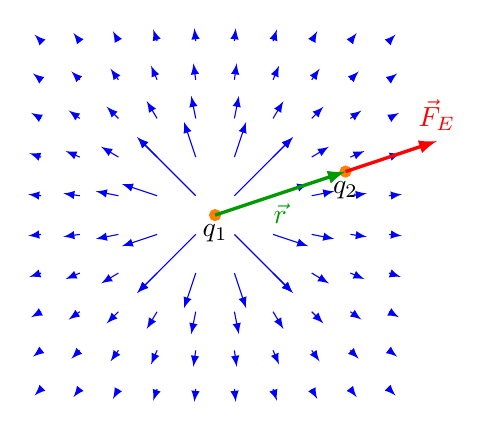
\begin{tikzpicture}
  \begin{axis}[
    xmin = -2, xmax = 2,
    ymin = -2, ymax = 2,
    axis equal image,
    xtick = {\empty},
    xticklabels = {\empty},
    ytick = {\empty},
    yticklabels = {\empty},
    view = {0}{90},
    height=6cm,
    samples = 10,
    color = blue,
    domain = -2:2,
    hide axis,
    clip = false,
    ]
    \addplot3[
      point meta = {pow(x^2+y^2,-0.05)},
      quiver = {
        u = {x/(x^2+y^2)},
        v = {y/(x^2+y^2)},
        scale arrows = 0.3,
        % every arrow/.append style={%
        %    -{Latex[scale={max(0.1,\pgfplotspointmetatransformed/1000)}]},
        % },
      },
      ->,
    ] {0};
    \coordinate (o) at (axis cs: 0,0);
    \coordinate (r) at (axis cs: 1.5,0.5);
    \draw[fill,orange] (axis cs: 0,0) circle[radius=2pt] node[below,black] {$q_1$};
    \draw[fill,orange] (r) circle[radius=2pt] node[below,black] {$q_2$};
    \draw[->,red,very thick] (r) -- ($(o)!1.7!(r)$) node[above] {$\vec{F}_E$};
    \draw[->,green,very thick] (o) -- node[below]{$\vec{r}$} (r);
  \end{axis}
\end{tikzpicture}
\end{document}
